\genHeader

When establishing a model-driven solution, \emph{model transformations} usually play a central and important role.
\marginpar{\emph{A Taxonomy of Model Transformations}}
Be it for specifying dynamic semantics (like for our learning box) or, more generally, for transforming a certain model to another model to achieve some goal (consistency, adding or abstracting from platform details, \ldots).  

There are many \emph{types} of model transformations and \cite{CH03,Mens_Gorp_2006} give a nice and detailed classification along a set of different dimensions. 
\marginpar{\emph{Model-to-Text\\ Transformations}}
In this chapter, we shall explore some of these dimensions and learn how \emph{model-to-text} transformations can be achieved with a nice mixture of \emph{string grammars} and \emph{graph grammars}. 

For the rest of the chapter a model transformation is to be regarded as:
\begin{displaymath}
 	\Delta: m_{src} \rightarrow m_{trg}
\end{displaymath}
where the source model $m_{src}$ is to be transformed to the target model $m_{trg}$.

$\Delta$ is \emph{endogenous}, if $m_{src}$ and $m_{trg}$ conform to the same metamodel.
\marginpar{\emph{Endogenous Model\\ Transformations}}
All the SDMs we have treated in the tutorial till now (for our learning box) are examples of endogenous transformations.

$\Delta$ is \emph{exogenous}, if $m_{src}$ and $m_{trg}$ are instances of different metamodels.
\marginpar{\emph{Exogenous Model\\ Transformations}}
In this chapter, we shall complement our learning box with a simple language for \emph{dictionaries}.
A dictionary is also used to learn new words but is more suitable to be used as a reference, i.e., one already knows most of the words and only specific words are looked-up now and then.
A learning box, on the other hand, is more geared towards supporting the actual memorization process.
Ergo?  One could start with a learning box and, when all words have been memorized, transform it to a personalized dictionary for future reference.
If one notices that too many words have been forgotten (typically after a long break or a lazy spell) a dictionary can be transformed \emph{back} to a learning box.
We shall see later on that this transformation is actually quite cool as one could, for example, use the history of cards or their difficulty level (fast cards are very simple) to either annotate entries in a dictionary or pre-place cards appropriately in a learning box. 

The learning box to dictionary transformation and vice-versa are examples of exogenous transformations.

$\Delta$ operates \emph{in-place}, if $m_{src}$ is destructively transformed to $m_{trg}$.
\marginpar{\emph{In-Place Model\\ Transformations}}
The SDMs for our learning box (e.g. grow or check) are examples for in-place transformations as they perform changes directly to a source model, transforming it destructively into the target model.


$\Delta$ is \emph{out-place} if $m_{src}$ is left intact and is not changed by the transformation that creates $m_{trg}$.
\marginpar{\emph{Out-Place Model\\ Transformations}}
The learning box to dictionary transformation and vice-versa are examples of out-place transformations.

Although endogenous + in-place is the natural case for SDMs (like for our learning box), we shall see in a moment that exogenous and/or out-place transformations can also be specified with SDMs.

%\vspace{1.5cm}
 
To twist your brain a bit here are a few interesting statements:
\begin{enumerate}
\item[$\blacktriangleright$] Out-place transformations can be endogenous or exogenous.

\item[$\blacktriangleright$] In-place transformations can usually\footnote{One can always think up crazy examples right?} only be endogenous.  Exogenous transformations are, consequently, always out-place.  Why? 
\end{enumerate}  

%\vspace{1.5cm}
   
$\Delta$ is further classified as \emph{horizontal} if $m_{src}$ and $m_{trg}$ are on the same \emph{abstraction level} and \emph{vertical} if they are not. 
\marginpar{\emph{Horizontal or\\ Vertical?}}

This last abstraction-level dimension is unfortunately a bit fuzzy but in a moment we shall explore and work on 
\marginpar{\emph{Abstraction Levels}}
different abstraction levels by establishing a textual concrete syntax for our dictionaries.

In the process we shall learn how graph transformations can be used, in combination with parser generators and template languages, to implement model-to-text and text-to-model transformations that are typically vertical (text is normally on a lower abstraction level than a model).  

Our learning box to dictionary transformation is, on the other hand, probably horizontal as the models represent the \emph{same} information, albeit differently, and can thus be considered to be on the same abstraction level.

\vspace{1.5cm}


In the following the \emph{Mo}flon \emph{C}ode \emph{A}dapter (\emph{Moca}) framework refers to:
\begin{enumerate}
 \item the approach we use to integrate string grammars, graph grammars and template languages, 
 \item how we separate the transformation into different modular steps, 
\marginpar{\emph{What is Moca?}}
 \item the usage of a generic and simple tree to consolidate different platforms, and 
 \item the actual tool support that acts as glue to hold all the different parts together.
\end{enumerate}
 
Fig.~\ref{fig:moca-overview} gives a ``big picture'' of what we plan to achieve in this chapter.
All explanations are integrated right in the figure so take your time and let it sink in.
We'll be zooming in on bits and pieces in the following sections to make things clearer and more concrete.

% \begin{figure}[htp]
% \begin{center}
%  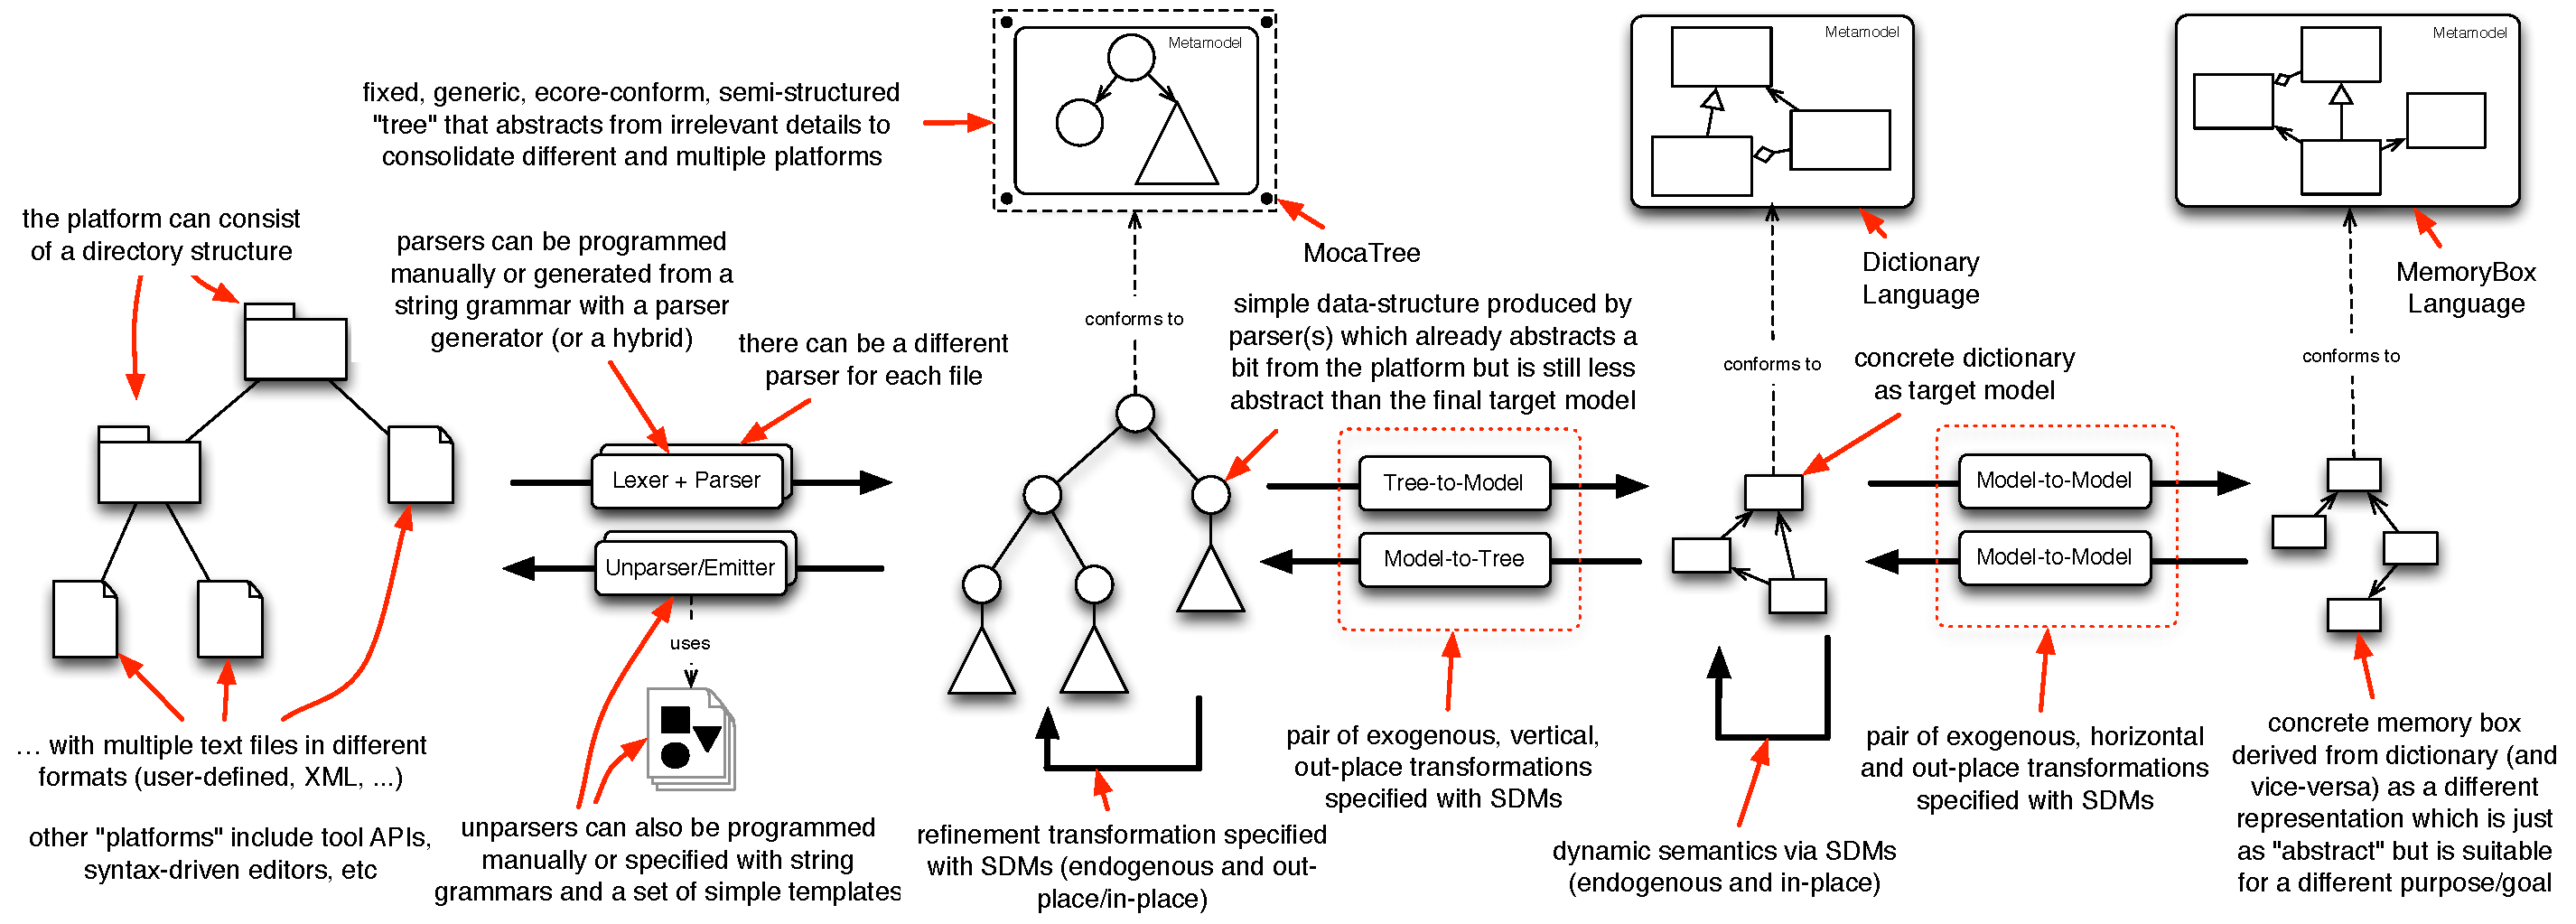
\includegraphics[angle=90, height=\textheight]{pics/moca/text-to-model}
%   \caption{Overview of model-to-text with the MOCA framework}
%   \label{fig:moca-overview}
% \end{center}
% \end{figure} 
